\section{Prelimiting Void-to-Absorber Test}
\label{sec:prelimiting_void_to_absorber}

In this section, the ``prelimiting'' procedure suggested by Kuzmin
\cite{kuzmin_FCT} is tested. The objective of prelimiting is to
cancel ``defective'' antidiffusive correction fluxes, i.e., those
which do not steepen the solution but instead flatten it. It
has been suggested that prelimiting the fluxes will mitigate
the formation of spurious plateaus in the solution; since these
spurious plateaus have been observed in the transient of the
void-to-absorber test problem described in Section \ref{sec:void_to_absorber},
this test problem is used in this section to examine the merits
of prelimiting.
Table \ref{tab:prelimiting_void_to_absorber_run_parameters}
shows the run parameters used to obtain these results, and Figure
\ref{fig:prelimiting_void_to_absorber} shows the results
for a number of different schemes. Spurious plateaus are observed
for Forward Euler (FE), which is inherently unstable, while
stable schemes such as Backward Euler (BE) and SSPRK33 do not
show any formation of spurious plateaus. Comparing the FE
scheme with and without prelimiting, these results show that
prelimiting has only a very small impact on the solution in this
case, and the procedure does not mitigate the formation of
spurious plateaus. Since prelimiting requires that the
low-order solution be computed when it is otherwise not needed,
these results do not justify the expense of the prelimiting
procedure.
%-------------------------------------------------------------------------------
\begin{table}[ht]\caption{Prelimiting Void-to-Absorber Test Run Parameters}
\label{tab:prelimiting_void_to_absorber_run_parameters}
\centering
\begin{tabular}{l l}\toprule
\emph{Parameter} & \emph{Value}\\\midrule
Number of Cells & $N_{cell} = 32$\\
End Time & $t = 0.75$\\
CFL Number & $\nu = 0.8$\\
\bottomrule\end{tabular}
\end{table}
%-------------------------------------------------------------------------------
\begin{figure}[ht]
   \centering
   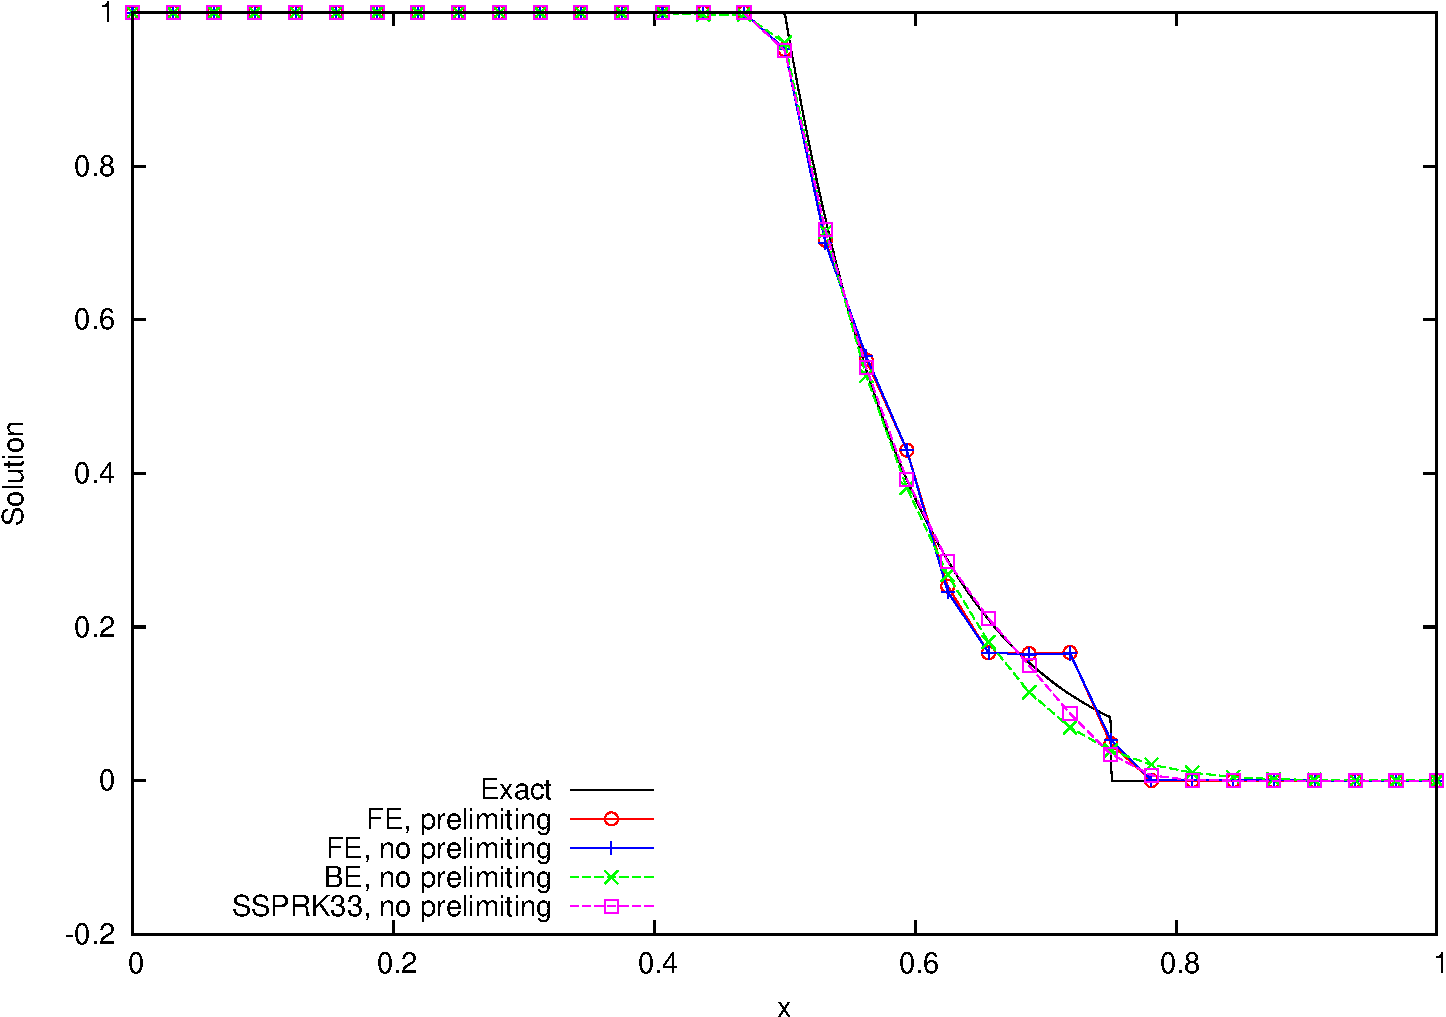
\includegraphics[width=\textwidth]
     {\contentdir/results/transport/prelimiting_void_to_absorber/prelimiting.pdf}
   \caption{Effect of Prelimiting on the Formation of Spurious Plateaus
      in the Void-to-Absorber Test Problem}
   \label{fig:prelimiting_void_to_absorber}
\end{figure}
%-------------------------------------------------------------------------------
